\newpage
\section{Auswertung}
\label{sec:auswertung}
\subsection{B-Feld Messung}
Da der Zeeman Effekt abhängig vom angelegten B-Feld ist un in diesem Versuchsaufbau nur der Spulenstrom zur Magnetfelderzeugung eingestellt werden kann muss zunächst der Zusammenhang zwischen Spulenstrom und Magnetfeld betrachtet werden.
Mit den Werten die wie in Abschnitt \ref{sec:BFeld} aufgenommen wurden wird ein linearer Fit und ein Fit eines Polynoms dritter Ordnung durchgeführt.\\
\begin{figure}[ht]
    \center
    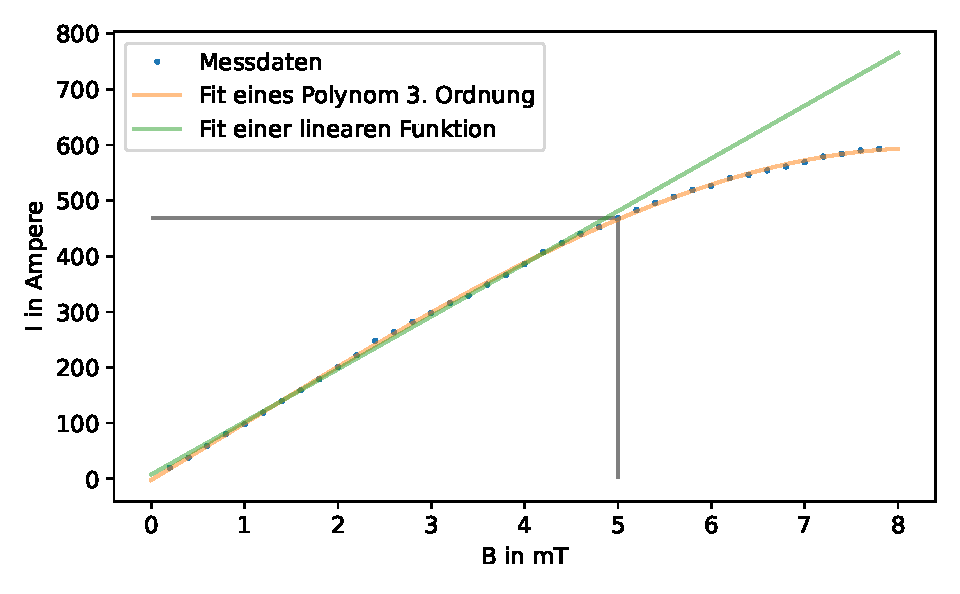
\includegraphics[width=0.65\textwidth]{plots/B_Feld.pdf}
    \caption{Die Feldstärke wird gegen den angelegten Spulenstrom aufgetragen. Im Bereich des grauen Kastens }
    \label{fig:B_Feld}
\end{figure}
Die beiden Fits basieren dabei auf folgenden Funktionen:
\begin{align*}
    B_1(I) &= aI^3+bI^2+cI+d\\
    B_2(I) &= mI+e
\end{align*}
Dabei ergeben sich die Parameter zu:
\begin{align*}
    a &= \SI[per-mode = fraction]{-0.62 +- 0.05}{\tesla \per \cubic \ampere}\\
    b &= \SI[per-mode = fraction]{1.7+-0.6}{\tesla \per \square \ampere}\\
    c &= \SI[per-mode = fraction]{100.8+-2.2}{\tesla \per \ampere}\\
    d &= \SI[per-mode = fraction]{-2.1+-2.1}{\tesla}\\
    \\
    m &= \SI[per-mode = fraction]{94.7+-0.9}{\tesla \per \ampere}\\
    e &= \SI[per-mode = fraction]{7.6+-2.6}{\tesla}\\ 
\end{align*}
\subsection{Der rote 643,8 nm-Übergang}
Im ersten Fall wird die Verschiebung der Interferenzmaxima durch den Zeeman Effekt beim roten Übergang mit der Wellenlänge \SI{643,8}{\nano\metre}.
Für die parallele Polarisation wurde keine Aufspaltung gemessen und für die senkrechte Polarisation wurden die Pixel zwischen den Maxima ausgelesen.
Als Unsicherheit für das Ablesen der Pixel wurden drei Pixel gewählt.
Die Aufspaltung wurde dabei nur bei der maximalen B-Feld-Stärke von \SI{590,86}{\milli\tesla} gesehen.
Die Aufspaltung zwischen den Maxima bei ausgeschaltetem B-Feld $\Delta s$ wird aus dem Bild ermittelt und mit dem selben verfahren auch die Aufspaltung der Maxima beim eingeschalteten B-Feld $\delta s$.
Aus diesen Werten lässt sich nun gemäß Formel \ref{eqn:lambda} die Verschiebung der Wellenlänge $\delta \lambda$ berechnen.
\begin{equation*}
    \delta \lambda_{rot,\sigma} = \SI{7.1(3)d-12}{\metre}
\end{equation*}
Diese Verschiebung wird gemittelt und gemäß der Gaußschen Fehlerfortpflanzung der Fehler bestimmt.
Durch Umstellen der Energieaufspaltung durch den Zeeman Effekt lässt sich aus den Wellenlängenverschiebungen damit der Landé-Faktor berechnen
\begin{equation*}
    g = \frac{\delta \lambda \cdot h c}{\mu_B B \lambda^2}
\end{equation*}
\begin{figure}
    \center
    
\includegraphics[width=0.65\textwidth]{bilder/bearbeitet/rot_senk.jpg}
    \caption{Das Interferenzmuster des roten Lichts bei senkrechter Polarisation und einem Magnetfeld von \SI{590,86}{\milli\tesla}}
    \label{fig:rot_senk}
\end{figure}
\begin{equation*}
    g_{rot} = \num{1.13+-0.06}.
\end{equation*}

\subsection{Der blaue 480,0nm-Übergang}
Für den blauen \SI{480}{\nano\metre} Übergang wird analog vorgegangen. 
Auch hier wurde eine Magnetfeldstärke von \SI{590,86}{\milli\tesla} verwendet um die Aufspaltung zu erzeugen.
Mit den Messwerten ergibt sich dabei eine Wellenlängenverschiebung von:
\begin{equation*}
    \delta \lambda_{blau,\sigma} = \SI{1.15(07) e-11}{\metre} 
\end{equation*}

\begin{figure}
    \center
    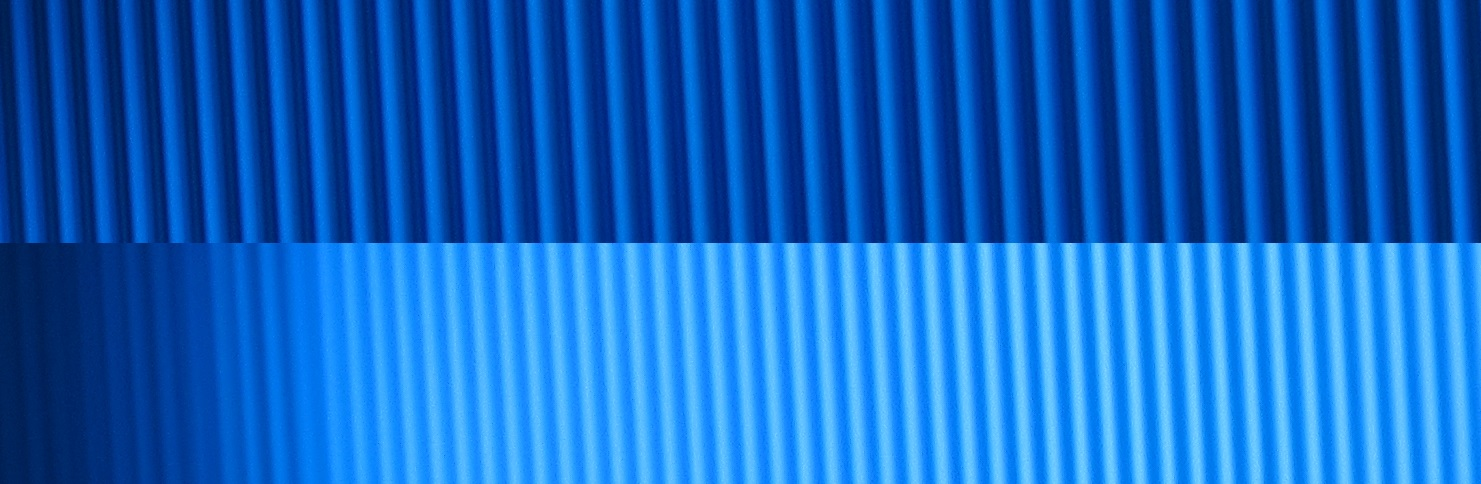
\includegraphics[width=0.65\textwidth]{bilder/bearbeitet/blau_senk.jpg}
    \caption{Das Interferenzmuster des blauen Lichts bei senkrechter Polarisation und einem Magnetfeld von \SI{590,86}{\milli\tesla}}
    \label{fig:blau_senk}
\end{figure}

\begin{equation*}
    g_{blau,\sigma} = \num{1.00+-0.06}
\end{equation*}



Für den blauen $\pi$ Übergang haben wir keine Messung durchgeführt, allerdings haben wir mit Ergebnissen aus vorherigen Versuchen arbeiten können.
Die Messung wurde mit einem Magnetfeld von circa \SI{1}{\tesla} durchgeführt und ergibt folgende Ergebnisse:
\begin{align*}
    \delta \lambda_{blau,\pi} = \SI{1.43(04) e-11}{\metre} \\
    g_{blau,\pi} = \num{0.738+-0.023}
\end{align*}

\begin{figure}
    \center
    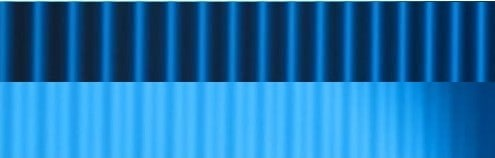
\includegraphics[width=0.65\textwidth]{bilder/bearbeitet/blau_parallel.jpeg}
    \caption{Das Interferenzmuster des blauen Lichts bei paralleler Polarisation und einem Magnetfeld von \SI{1}{\tesla}}
    \label{fig:blau_parallel}
\end{figure}